\subsubsection{Коррекция увязки по глубине}
\par
При проведении анализа данных ПГИ, полученных от датчиков в каротажной сборке приборов необходимо, во-первых, привязать показания по длине ствола скважины, и, во-вторых, синхронизировать сигналы от датчиков, поскольку приборы в сборке расположены на некотором расстоянии друг от друга, обычно не более нескольких метров. Пример каротажной сборки приборов показан на рис.\ref{fig:log_example}. Для привязки по стволу используются гамма-каротаж совместно с локатором муфт \cite{169255} и другие решения. Синхронизация сигналов производится предобработкой «сырых» данных на основе информации о расположении датчиков друг относительно друга и их технических характеристик. В идеале ожидается, что все события в анализируемых временных рядах точно привязаны к истинным значениям координаты траектории скважины. 

\begin{figure}[H]
\centering
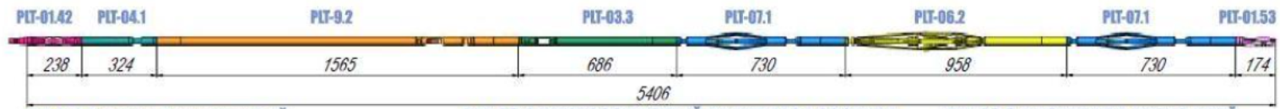
\includegraphics[width=1\textwidth]{DM/log_example.png}
\caption{Пример расположения датчиков в каротажной сборке. Здесь PLT-X - различные приборы; расстояния между ними указаны в миллиметрах.}
\label{fig:log_example}
\end{figure}

\par
Тем не менее, на первом этапе работы с полевыми данными (предоставленными нам уже после указанной предобработки) было решено проверить, насколько ситуация близка к идеальной. Корреляционный анализ показал, что рассинхронизация может превышать разумные погрешности, например 0.5м. Поэтому мы разработали и реализовали алгоритм предварительной синхронизации полевых данных. Отметим, что причинами рассинхронизации могут быть как технические сбои приборов и записывающей/считывающей аппаратуры, так и человеческий фактор. Это, вероятно, порождает ошибки в стандартных алгоритмах предобработки. Поэтому дополнительное использование корреляционного анализа позволяет распознать участки траектории с рассинхронизацией и устранить ее.
\par
В предложенном алгоритме синхронизации производится автоматическая коррекция относительных сдвигов датчиков, которые уже не обязательно будут соответствовать реальным расстояниям между ними в приборе.

\paragraph{Постановка задачи}
\par
Предположим, что имеется $N$ датчиков $\alpha_n,\;n\in[1,N]$, расположенных на некотором отрезке (сборка приборов) и генерирующих сигналы – последовательности по времени. Для удобства можно представить, что отрезок закреплен, а скважина движется относительно него. Отметим, что координата по времени однозначно пересчитывается в координату по стволу скважины через скорость движения. 
\par
Назовем вектором сдвигов набор значений $(\alpha_n,s_n),\;n\in[1,N]$, где для каждого датчика $\alpha_i,\;i\in[2,N]$ указан сдвиг $s$ показаний этого датчика относительно опорного датчика $\alpha_1$ такой, что $-10\text{м}<s_i<10\text{м}$ и $s_1=0$.
\par
В идеале все сдвиги равны нулю (датчики находятся в одной точке). В реальности они разнесены, отсюда возникает рассинхронизация последовательностей сигналов от датчиков. Нам надо найти оптимальный вектор сдвига с учетом разной физики и зашумленности сигналов. Такой сдвиг с противоположным знаком должен обеспечить синхронизацию последовательностей.

\paragraph{Алгоритм}
\par
Для разработки алгоритма анализировались данные по горизонтальной скважине Х45. На устойчивость работы алгоритма влияет много факторов, включая разную физику сигналов (температура, акустический шум, скорость флюида, фаза флюида и т.д.), зашумленность и др. Чтобы уменьшить влияние этих факторов, был выбран близкий к горизонтальному участок траектории, так как показания датчиков меньше подвержены искажениям, вызванных физической перестройкой течения в местах изменения наклона скважины. ми изменений траектории событиями. В данном случае длина участка составляла 300 метров (3000 точек). В качестве опорного датчика использовался сигнал показаний глубины – TVD (true vertical depth). 
\par
\textit{Шаг 1}. Назовем оптимальным сдвигом между двумя массивами показаний $A_1$ и $A_2$ число $s_{12}= s(A_1,A_2)$ такое, что:
\begin{equation}
    s_{12}=\arg\max_{-10\text{м}\leq s\leq10\text{м}} \left(corr(A_1,A_2-s)\right),
\end{equation}
то есть такой сдвиг, применение которого к массивам $A_1,A_2$ позволит достичь максимального коэффициента корреляции Пирсона между ними.
\par
Оптимальный сдвиг можно оценить перебором возможных значений сдвигов в диапазоне $[-10\text{м},10\text{м}]$. В первом шаге алгоритма для каждой пары показаний датчиков вычисляется оптимальный сдвиг, результатом вычисления является антисимметричная матрица 1 размера $N\times N$ (рисХ). 
\par
Отсутствующие значения в ячейках матрицы 1 означают, что максимум коэффициента корреляции был достигнут на границах рассматриваемого участка $\pm10\text{м}$. Так как длина колонны обычно не превышает $10$м в длину, такие максимумы корреляции нефизичны, то есть, на рассматриваемом интервале траектории данные не имеют заметной корреляции, и алгоритм «поймал» корреляцию уже не связанных друг с другом событий.
\par
Из-за большого количества «пустых значений» в данном случае полученная матрица 1 состоит из одного столбца и одной строки – то есть необходимые взаимные сдвиги можно получить, просто взяв эти столбец или строку. Однако, такой вид матрицы не гарантируется: в общем случае может нарушаться аддитивность оптимальных взаимных сдвигов. Поэтому автоматическое определение оптимального вектора сдвигов предполагает дополнительный шаг.
\par
\textit{Шаг 2}. Если бы отсутствовали любые сдвиги между датчиками, матрица 1 состояла бы только из нулей. Будем к этому стремиться. Назовем оптимальным вектором сдвигов такой вектор сдвигов $(\alpha_n,s_n)^{opt},\;n\in[1,N]$, при применении которого к данным матрица 1 была бы минимальной по евклидовой норме, то есть:
\begin{equation}
    S^{opt}=\arg\min_{s\in[-10,10]^N}\sum_{i,j}(M_{ij})^2
\end{equation}
При вычислении нормы матрицы отсутствующие значения полагаются равными нулю.
Для оптимизации $L_2$-нормы матрицы $M$ предлагается следующий алгоритм:
\begin{itemize}
    \item[]$S^0=[0]\times N$ – изначально нулевой вектор сдвигов,
    \item[]$i=1$ – номер строки матрицы $M$,
    \item[]$k=0$ – номер итерации,
    \item[]$\varepsilon=10^{-3}$ – регулируемый критерий останова сходимости,
    \item[]$M^0=M$ – полученная на шаге 1 матрица попарных сдвигов,
    \item[]$F^0=L_2(M)=\sum_{i,j}(M_{ij})^2$ – начальное значение минимизируемой нормы матрицы.
    \item[] while $F^k>\varepsilon$:
    \begin{itemize}
        \item[]$m=\frac{1}{N}\sum_{n=1}^N M_{in}$ 
        \item[]$S_i^k=m$
        \item[]Нулевая матрица $T^k$  размера NxN заполняется следующим образом:
        $$\forall i\in[1,..,N],\;\forall j\in[1,...,i-1,i+1,...,N]\rightarrow T_{ij}^k=m,\; T_{ji}^k=-m$$
        \item[]$M^k=M^{k-1}-T^k$
        \item[]$k=k+1$
        \item[]$i=i+1$ если $i<N$, иначе $i=0$
        \item[]$F^k=L_2(M^k)$
    \end{itemize}
\end{itemize}
\par
Таким образом, на каждой итерации из соответствующей строки матрицы вычитается ее среднее; к соответствующему столбцу добавляется это среднее для сохранения антисимметричности; вычисленное среднее добавляется к изначально пустому вектору сдвигов.
\par
На рассматриваемом примере оптимизируемый функционал в результате алгоритма уменьшился с $F^0=320.5$ до $F^K=2.5\times 10^{-4}$ за $K=10$ итераций. Результаты на примере некоторых данных скважины X45 показаны на следующих рисунках: создание и преобразование матрицы сдвигов на рис.\ref{fig:shift_matrices}, предложенная схема расположения датчиков на рис.\ref{fig:shift_log} и демонстрация сдвига данных на рис.\ref{fig:shift_signals}.

\begin{figure}[H]
\centering
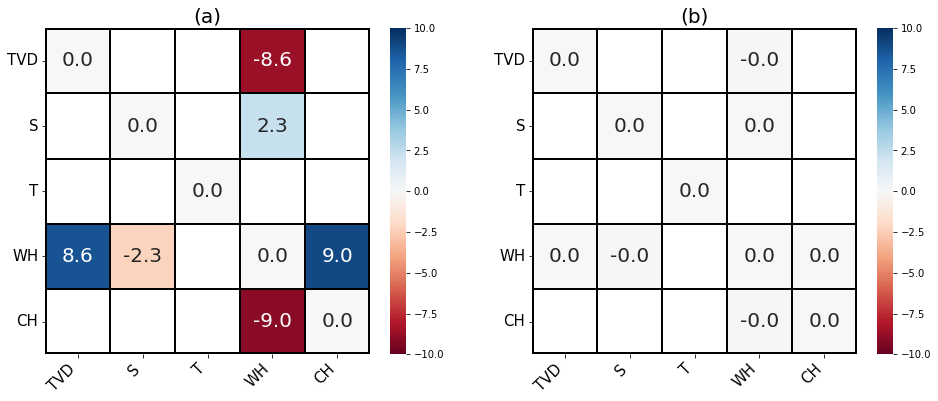
\includegraphics[width=0.8\textwidth]{DM/shift_matrices.png}
\caption{Матрицы попарных оптимальных сдвигов. (a) - вариант до оптимизации, (b) - результат после минимизации $L_2$-нормы. Видно, что удалось достичь идеального случая - с определенной точностью все несоответствия стали нулевыми.}
\label{fig:shift_matrices}
\end{figure}

\begin{figure}[H]
\centering
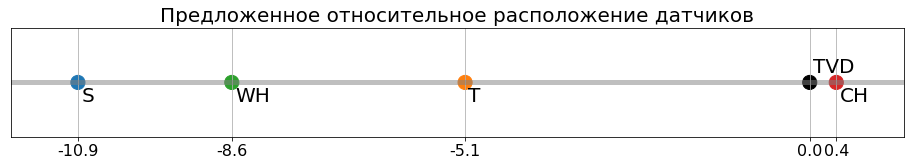
\includegraphics[width=0.8\textwidth]{DM/shift_log.png}
\caption{Примерная предложенная схема сдвига датчиков по полученным значениям. Здесь сдвиги отцентрированы относительно датчика глубины - TVD.}
\label{fig:shift_log}
\end{figure}

\begin{figure}[H]
\centering
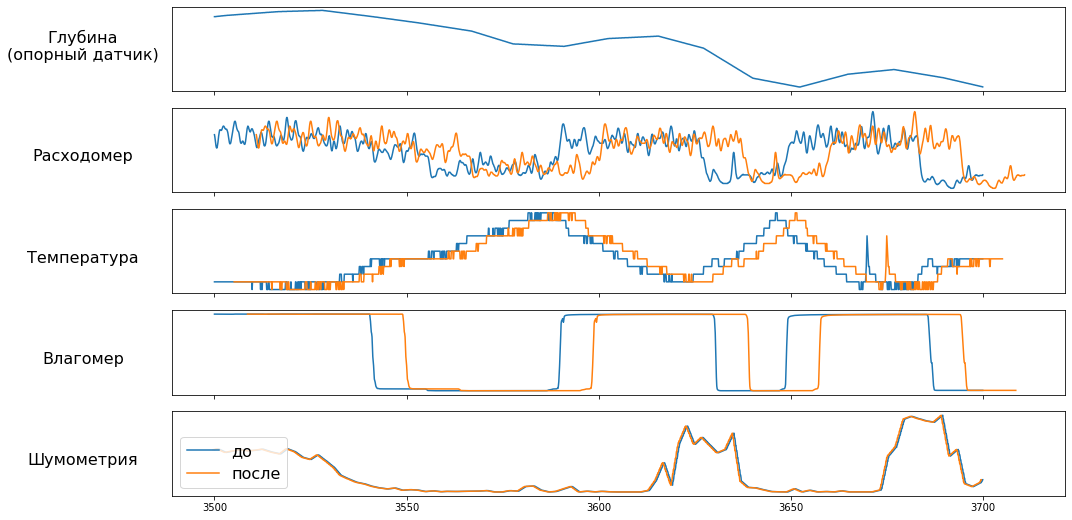
\includegraphics[width=0.9\textwidth]{DM/shift_signals.png}
\caption{Демонстрация того, как полученные сдвиги повлияли на визуальное соответствие датчиков.}
\label{fig:shift_signals}
\end{figure}

\par
Можно продемонстрировать необходимость выбора наиболее горизонтального участка траектории для анализа. На рисунках \ref{fig:shift_matrices_bad},\ref{fig:shift_log_bad},\ref{fig:shift_signals_bad} изображены матрицы получения оптимального вектора сдвигов с использованием всей траектории – порядка километра. На протяжении траектории происходит множество событий, которые вносят шум в данные. Из-за этого не получается достичь удовлетворительных результатов – оптимизация матрицы на шаге 2 мало меняет ситуацию (несмотря на то, что оптимизируемый функционал уменьшился с А до В), и применение полученных сдвигов не соответствует ранее полученным результатам и в принципе тому, что могло бы быть результатом ручной работы.

\begin{figure}[H]
\centering
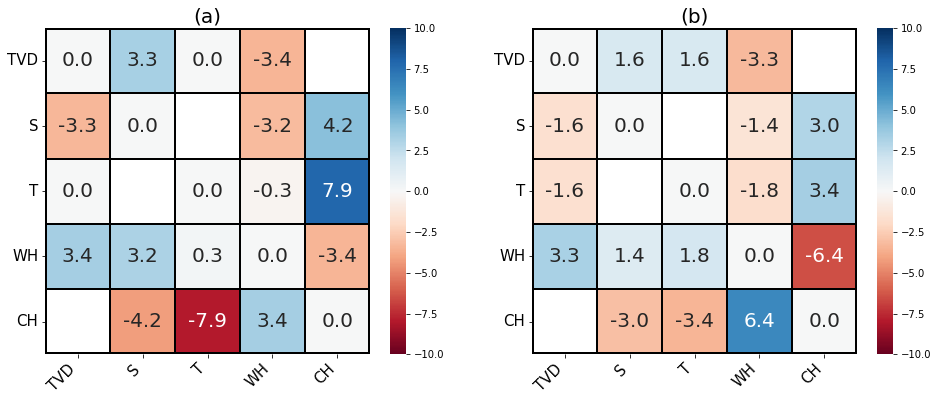
\includegraphics[width=0.8\textwidth]{DM/shift_matrices_bad.png}
\caption{Матрицы аналогично предыдущему случаю. Видно, что на втором шаге (b)  не удалось достичь идеального результата - нулевой матрицы; это показывает, что диапазон траектории для анализа был выбран неверно.}
\label{fig:shift_matrices_bad}
\end{figure}

\begin{figure}[H]
\centering
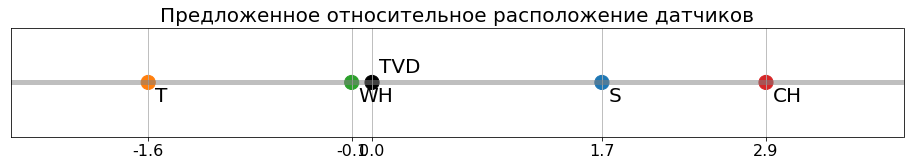
\includegraphics[width=0.8\textwidth]{DM/shift_log_bad.png}
\caption{Полученные сдвиги не совпадают с тем, что мы получили на предыдущем этапе.}
\label{fig:shift_log_bad}
\end{figure}

\begin{figure}[H]
\centering
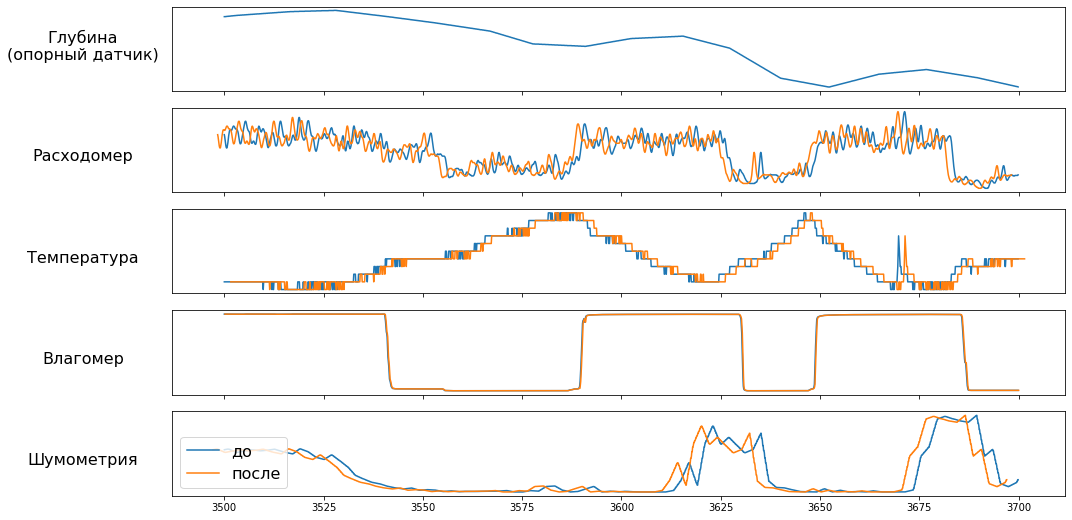
\includegraphics[width=0.9\textwidth]{DM/shift_signals_bad.png}
\caption{Видно, что алгоритм почти ничего не поменял в данных - и визуального совмещения пиков сигналов не вышло.}
\label{fig:shift_signals_bad}
\end{figure}
